\documentclass[12pt]{article}
\usepackage[margin = 1in]{geometry}
\usepackage{amsmath, amssymb, amsthm, graphicx}
\usepackage{enumerate}
\usepackage[all]{xy}
\usepackage{mathrsfs}

%%%%%%%%%%%%%% COLOR COMMENTS! %%%%%%%%%%%%%%%
\usepackage{color}
\newcommand{\dzb}[1]{{\color{blue} \sf
    $\spadesuit\spadesuit\spadesuit$ DZB: [#1]}}
\newcommand{\reword}[1]{{\color{red} \sf $\spadesuit\spadesuit\spadesuit$ reword: [#1]}}

% changed above definition to make comments disappear
%\newcommand{dzb}[1]{}
%\newcommand{reword}[1]{}

% Color names: http://en.wikibooks.org/wiki/LaTeX/Colors#The_68_standard_colors_known_to_dvips
\usepackage[usenames,dvipsnames]{xcolor}
\newcommand{\note}[1]{{\color{BurntOrange} $\blacktriangle\blacktriangle$\sf Note: [#1]}}

\newcommand{\F}[0]{\mathbb{F}}
\newcommand{\tr}[0]{\operatorname{tr}}
\newcommand{\wt}[1]{\widetilde{#1}}
\newcommand{\frob}[0]{\operatorname{Frob}}
\newcommand{\card}[0]{\#}
\newcommand{\pmat}[4]{\begin{pmatrix}#1 & #2 \\ #3 & #4\end{pmatrix}}
\newcommand{\pderiv}[2]{\frac{\partial #1}{\partial #2}}
\newcommand{\Ov}{\mathcal{O}_{v}}
\newcommand{\Ok}{\mathcal{O}_{K}}
\newcommand{\Q}{\mathbb{Q}}
\newcommand{\Z}{\mathbb{Z}}
\newcommand{\C}{\mathbb{C}}
\newcommand{\leg}[2]{\left(\frac{#1}{#2}\right)}
\newcommand{\calO}{\mathcal{O}}
\newcommand{\frakp}{\mathfrak{p}}
\newcommand{\frakq}{\mathfrak{q}}
\newcommand{\mf}[1]{\mathfrak{#1}}
\newcommand{\nm}{\operatorname{N}_{K/\Q}}
\newcommand{\Cl}{\operatorname{Cl}}
\newcommand{\oo}{\mathcal{O}}
\newcommand{\sgn}{\operatorname{sgn}}
\newcommand{\Gal}{\operatorname{Gal}}
\newcommand{\cl}{\overline}
\newcommand{\mc}[1]{\mathcal{#1}}
\newcommand{\Cc}{\mathcal{C}}
\newcommand{\Dc}{\mathcal{D}}
\newcommand{\raym}{\mathcal{C}^{\frakm}_K}
\newcommand{\frakr}{\mathfrak{r}}
\newcommand{\Spec}{\text{Spec} \ }
\newcommand{\Hom}{\text{Hom}}
\newcommand{\ord}{\text{ord}}
\newcommand{\scr}[1]{\mathscr{#1}}
\newcommand{\R}{\mathbb{R}}
\newcommand{\Nm}{\text{Nm}}
\newcommand{\A}{\mathbb{A}}
\newcommand{\ti}{\times}
\newcommand{\Hbb}{\mathbb{H}}
\newcommand{\ol}[1]{\overline{#1}}
\newcommand{\ul}[1]{\underline{#1}}
%\newcommand{\leg}[2]{\left(\frac{ \# 1}{\# 2} \right)}

\DeclareMathOperator{\GL}{GL}
\DeclareMathOperator{\SL}{SL}
\DeclareMathOperator{\Frob}{Frob}
\DeclareMathOperator{\ab}{ab}
\DeclareMathOperator{\cyc}{cyc}
\DeclareMathOperator{\N}{N}
\DeclareMathOperator{\Ver}{Ver}
\DeclareMathOperator{\Art}{Art}
\DeclareMathOperator{\Spl}{Spl}
\DeclareMathOperator{\sep}{sep}
\DeclareMathOperator{\Stab}{Stab}
\DeclareMathOperator{\Sp}{Sp}
\DeclareMathOperator{\SO}{SO}
\DeclareMathOperator{\SU}{SU}
\DeclareMathOperator{\PGL}{PGL}
\DeclareMathOperator{\Mat}{Mat}
\DeclareMathOperator{\Tr}{Tr}
\DeclareMathOperator{\End}{End}
\DeclareMathOperator{\Ad}{Ad}
\DeclareMathOperator{\Aut}{Aut}
\DeclareMathOperator{\argmax}{argmax}

\newtheorem{thm}{Theorem}
\newtheorem{lemma}[thm]{Lemma}
\newtheorem{defn}[thm]{Definition}
\newtheorem{prop}[thm]{Proposition}
\newtheorem{cor}[thm]{Corollary}
\newtheorem{ex}[thm]{Example}
\newtheorem{crit}[thm]{Criterion}


\theoremstyle{remark}
\newtheorem{rem}[thm]{Remark}

\makeatletter
\def\imod#1{\allowbreak\mkern5mu({\operator@font mod}\,\,#1)}
\makeatother

\widowpenalty=1000
\clubpenalty=1000

\title{CS181 Assignment 4}
\author{Ashok Cutkosky and Tony Feng}


\begin{document}
\maketitle

\subsection*{Problem 1.} (a) According to the graph depicted below, we need to describe the following intermediate probabilities: 
$P(RD), P(MAI), P(NAI \mid MAI), P(VP \mid RD), P(SMOS \mid VP)$, and $P(VRAS \mid VP)$. 
\[
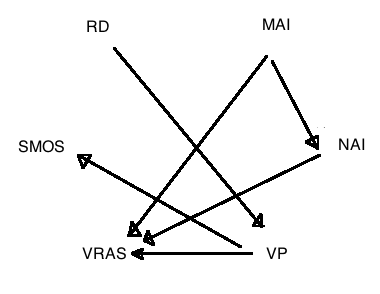
\includegraphics[scale = 0.75]{4_1_1.png}
\]
We parametrize the noise by a uniform random variable $\cal{U}(a,b)$ on interval $(a,b)$. 
\begin{itemize}
\item First, we assume that $P(RD) = 0.2, P(MAI) = 0.5$. 
\item Next, we assume that $P(VP \mid RD)$ is given by the following table
\[
\begin{tabular}{|l|l|l|}
\hline
& RD = 1 & RD = 0 \\
\hline
P(VP = 1) & $ 0.9 $& 0.0 \\
\hline
\end{tabular}
\]


$P(SMOS \mid VP) $ is given by the following table 
\[
\begin{tabular}{|l|l|l|}
\hline
& VP = 1 & VP = 0 \\
\hline
P(SMOS = 1) & $0.9$ & 0.0 \\
\hline
\end{tabular}  
\]
and $P(NAI \mid MAI)$ is given by the following table
\[
\begin{tabular}{|l|l|l|}
\hline
& MAI = 1 & MAI = 0 \\
\hline
P(NAI = 1) & 0.1 & 0.9 \\
\hline
\end{tabular}  
\]
\item Finally, we assume that $P(VRAS)$ is given by the following table:
\[
\begin{tabular}{|l|l|l|l|l|l|}
\hline
(VP, MAI, NP)& (0,*,*)& (*, 0, 0) & (1,1,0) or (1,0,1) & (1,1,1) \\
\hline
P(VRAS = 1) & 0  & 0 & $ 0.7+ \mathcal{U}(-\alpha_0, \alpha_1) $ & $0.9 + \mathcal{U}(-\beta_0, \beta_1) $\\
\hline
\end{tabular}  
\]
\end{itemize}
Observe that the $\alpha_i$ and $\beta_i$ parametrize the probability of the antivirus detecting the virus. \\

\noindent (b) Above, we assumed that SMOS (silly messages on screen) was independent of RD (recent download) conditioned on VP (virus present). However, it could be argued that one could have SMOS, e.g. from the ads that tend to inhabit untrusted sites, without actually having a virus. In this case, we should add an edge from RD to SMOS, since we can imagine that RD indicates browsing of the kind of sites that would pop up such silly messages. 

We chose not to include this edge for the sake of simplicity, since we expect the majority of silly messages to come from viruses. The problem at hand seems to be that of modeling the virus process, and we can adjust our definition of ``silly messages'' to be pretty sure that they correspond to viruses. \\

\noindent (c) Here is our new graph.
\[
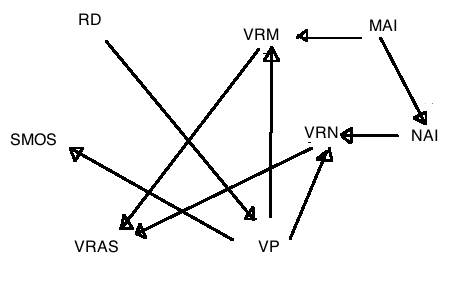
\includegraphics[scale=0.8]{4_1_2.png}
\]
The things to change are $P(VRM \mid MAI , VP), P(VRN \mid NAI, VP)$, and $P(VRAS \mid ...)$. We are modifying our parametrization slightly so that $P(VRM \mid MAI, VP) = 0.7 + \mathcal{U}(-\alpha_0, \alpha_1)$ and $P(VRN \mid NAI, VP) = 0.75 + \mathcal{U}(-\beta_0, \beta_1) $, and $VRAS = 1$ if either $VRM$ or $VRN = 1$. \\

\noindent (d) Well, introducing these nodes allows greater flexibility of expression in the modeling process because it allows us to separate the dependencies on the two different antivirus programs. For instance, the graph lets us think about the probability that McAfee detects a virus and the probability that Norton detects a virus separately. 

Whether or not this is beneficial to the modeling process depends on our specific goals and situation. It is conceivable that this extra complexity could lead us towards overfitting. Note also that it could already be captured by the parameters of the simpler model, so one could argue that there is not, strictly speaking, more information in this second model. 

\subsection*{Problem 2} (a) For graph (a), there are no such variables. For graph (b), the independent variables are $F,C$. This was determined using the algorithm for detecting $d$-separation on page $75$ of Koller and Friedman, \textit{Probabilistic Graphical Models.} For the first graph, $G$ and $D$ were marked, and none of the vertices are blocked. For the second, $G,D,B$ are marked, and $C,F$ are blocked at $I$. \\

\noindent (b) For graph (a), $P(A,B,C,D,E,F,G,H,I)$ is 
\[
P(G) P(H) P(I \mid G,H) P(D \mid G) P(E \mid G) P(F \mid H) P(B \mid D) P(C \mid E,F) P(A \mid B,C).
\]
For graph (b), $P(A,B,C,D,E,F,G,H,I)$ is
\[
P(B) P(C) P(A) P(D \mid B) P(E \mid B) P(F \mid C) P(G \mid A,D) P(H \mid D,E) P(I \mid E,F) P(J \mid G).
\]

\noindent (c) See the image. We have labeled the functions at each square to give the right probability distribution. For graph (a),
\[
\includegraphics[width=.75\textwidth]{4_2_1.png}
\]
For graph (b),
\[
\includegraphics[width=\textwidth]{4_2_2.png}
\]
\\

\noindent (d) See the image. Since the Undirected Graphical Models embed fully faithfully into the Factor Graphs, we do not need to label the functions again (they are the same). For graph (a),
\[
\includegraphics[width=.7\textwidth]{4_2_3.png}
\]
For graph (b),
\[
\includegraphics[width=.75\textwidth]{4_2_4.png}
\]
\subsection*{Problem 3} (a) 
\[
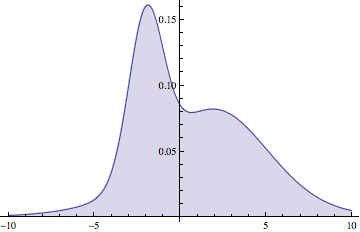
\includegraphics[scale=1]{4_3_1.png}
\]
(b) We draw in two steps. 
\begin{enumerate}
\item First draw randomly from the discrete distribution to determine from which Gaussian to draw: with probability $0.2$ we draw from the first, with probability $0.3$ we draw from the second, and with probability $0.5$ we draw from the third. 
\item Second draw from the Gaussian distribution determined in Step 1. 
\end{enumerate}
Using this algorithm, we produced the following histogram. 
\[
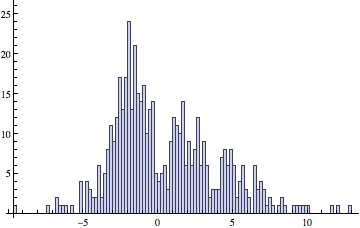
\includegraphics[scale=1]{4_3_2.png}
\]
(c) We chose to use the envelope function $g(x) = 2\mathcal{N}(\mu = 0, \sigma = 5.1)$, depicted below. 
\[
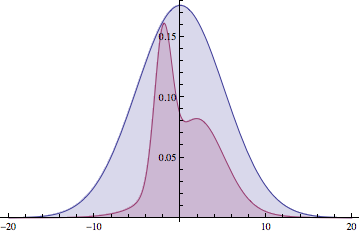
\includegraphics[scale=1]{4_3_3.png}
\]
For let us discuss why it actually fits the condition $g(x)> f(x)$ for all $x$. A challenge with Gaussian distributions is to bound the tail. Our examples has a greater variance than any of the constituent Gaussians in $f$, so its tail will dominate their tails for large $x$ (consider the term $e^{-x^2/\sigma^2}$, where $\sigma$ controls the rate of exponential decay). 

We wanted something with small tails to mold the small tails of $f$ closely, and another Gaussian was the natural choice. From there, it was a matter of tweaking the parameters. 

Note that our envelop has volume $2.25$, so we expect a success rate of $1/2.25$. Indeed, we need $1143$ trials for $500$ samples, and for comparison $1143/2.25 = 508$. Here is the histogram. 
\[
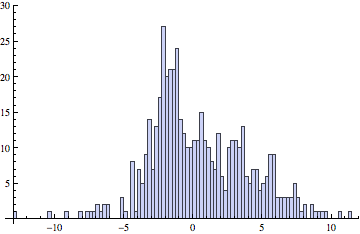
\includegraphics[scale=1]{4_3_4.png}
\]
(b) See below for the acceptance rates for various standard deviations.
\[
\begin{tabular}{|l|l|}
\hline
$\sigma$ & Number accepted \\
\hline
$0.25$  & 484 \\
$0.50$ & 446 \\
$0.75$ & 470 \\
$1.00$  & 439 \\
$1.25$ & 426 \\
$1.50$ & 408 \\
$1.75$ & 388 \\
$2.00$ & 402 \\
$2.25$ & 353 \\
\hline
\end{tabular}
\]
We have depicted, below, the histogram for Gaussians with variance $\sigma = 0.25, 0.5, \ldots, 2.0$. 
\begin{figure}[!h]
\includegraphics[scale=0.6]{4_3_5.png}
\includegraphics[scale=0.6]{4_3_6.png} 
\includegraphics[scale=0.6]{4_3_7.png}
\includegraphics[scale=0.6]{4_3_8.png}
\includegraphics[scale=0.6]{4_3_8.png}
\includegraphics[scale=0.6]{4_3_10.png}
\includegraphics[scale=0.6]{4_3_11.png}
\includegraphics[scale=0.6]{4_3_12.png}
%\includegraphics[scale=1]{4_3_13.png}


%\includegraphics[scale=1]{4_3_14.png}\\
%\includegraphics[scale=1]{4_3_15.png}\\

\end{figure}

For small of $\sigma$, the algorithm doesn't appear to have converged well to the desired distribution. The ``exploration rate'' is too low, and the Markov chain tends to move in small steps. The steps are concentrated in high density areas, so the rejection rate is lower. 

As $\sigma$ increases, we see better convergence to the distribution, and a slightly higher rejection rate. 

When $\sigma$ is too large, however, the resolution of the Markov process is wrong again and we expect to see excessively high rejection rates and clumping. 
\end{document}



